The Fox-Wolfram moments, introduced in \Cref{sec:modified_fox_wolfram_moments} were shown to bias the photon-energy spectrum.
This issue, and the fact that a better separation can be calculated if considering only certain subsets of particle momenta and energies in the event,
motivated the introduction of modified Fox-Wolfram moments, also known as Kakuno-Super-Fox-Wolfram moments.
They were originally introduced by the Belle collaboration in 2003 \cite{Belle:2003fgr} for charmless $B$ decay studies.
Modified Fox-Wolfram moments are defined in terms of a set of momenta $\vec{p}^{s}_i$ that belong to a $B$-meson candidate.
Another subset of momenta for different other particles not used in the reconstruction $\vec{p}^{o}_{jx}$, where $x$ represents a category.
The categories in question are charged particles ($c$), neutrals particles ($n$), and missing momentum ($m$).
With this in mind, linear modified Fox-Wolfram moments 
\begin{equation}
    H_{x,l}^{so} = \frac{1}{N} \sum_i \sum_{jx} Q^{l}_{ij}|p^o_{jx}|P_l(cos\theta_{i,jx}),
\end{equation}
and quadratic modified Fox-Wolfram moments
\begin{equation}
    R_{l}^{oo} = \frac{1}{N^2} \sum_i \sum_j Q^{l}_{ij} |p^o_i||p^o_j|P_l(\cos\theta_{i,j}),
\end{equation}
are defined.
Here, 
\begin{itemize}
\item $N\equiv 2(\sqrt{s}-E^{*}_B)$ is a normalisation factor defined in terms of the collisions center-of-mass energy and the $B$ meson energy in the center-of-mass frame;
\item $\sum_i$ runs over all particles used in the reconstruction of the $B$ candidate;
\item $\sum_j(x)$ runs over all other (or a category $x\in{c,n,m}$ of) particles in the event;
\item $Q^{l}_ij$ is the product of the charges of candidates corresponding to $i$ and $j$ if $l$ is odd, otherwise 1;
\item $q_{i(x)}$ are the charges of candidates corresponding to momentum $\vec{p}_{i(x)}$;
\item $\theta_{i,j(x)}$ is the angle between $\vec{p}_i$ and $\vec{p}_{j(x)}$;
\item $P_l$ are the Legendre polynomials.
\end{itemize}
As the charge for $x\in\{n,m\}$ is considered 0, they do not have odd $H^{so}_{\ell}$ moments.
Two additional variables are included: the transverse momentum of the event, $\vec{p}_{T}$ and the missing mass of the event $m_{\mathrm{miss}}^2$,
yielding a total of 18 variables suitable for continuum suppression.
In this analysis, they are calculated in terms of the tag-$B$ meson candidate and shown in
\Cref{fig:Btag_KSFW_hso00,fig:Btag_KSFW_hso01,fig:Btag_KSFW_hso02,fig:Btag_KSFW_hso03,fig:Btag_KSFW_hso04,fig:Btag_KSFW_hso10,fig:Btag_KSFW_hso12,fig:Btag_KSFW_hso14,fig:Btag_KSFW_hso20,fig:Btag_KSFW_hso22,fig:Btag_KSFW_hso24,fig:Btag_KSFW_hoo0,fig:Btag_KSFW_hoo1,fig:Btag_KSFW_hoo2,fig:Btag_KSFW_hoo3,fig:Btag_KSFW_hoo4,fig:Btag_KSFW_et,fig:Btag_KSFW_mm2}.
Six\footnote[1]{Due to an unfortunate mistake in the analysis code, $H_{c,1}^{so}$ and $H_{c,3}^{so}$ were not included in the \BDT training, although they did pass the \textbf{Test~1} selection criteria.
Therefore, strictly speaking `only 4' variables passed the human-error selection.
}
moments pass the requirements of \textbf{Test~1}.

\begin{figure}[htbp!]
    \centering
    \subcaptionbox{\label{fig:Btag_KSFW_hso00}}{
        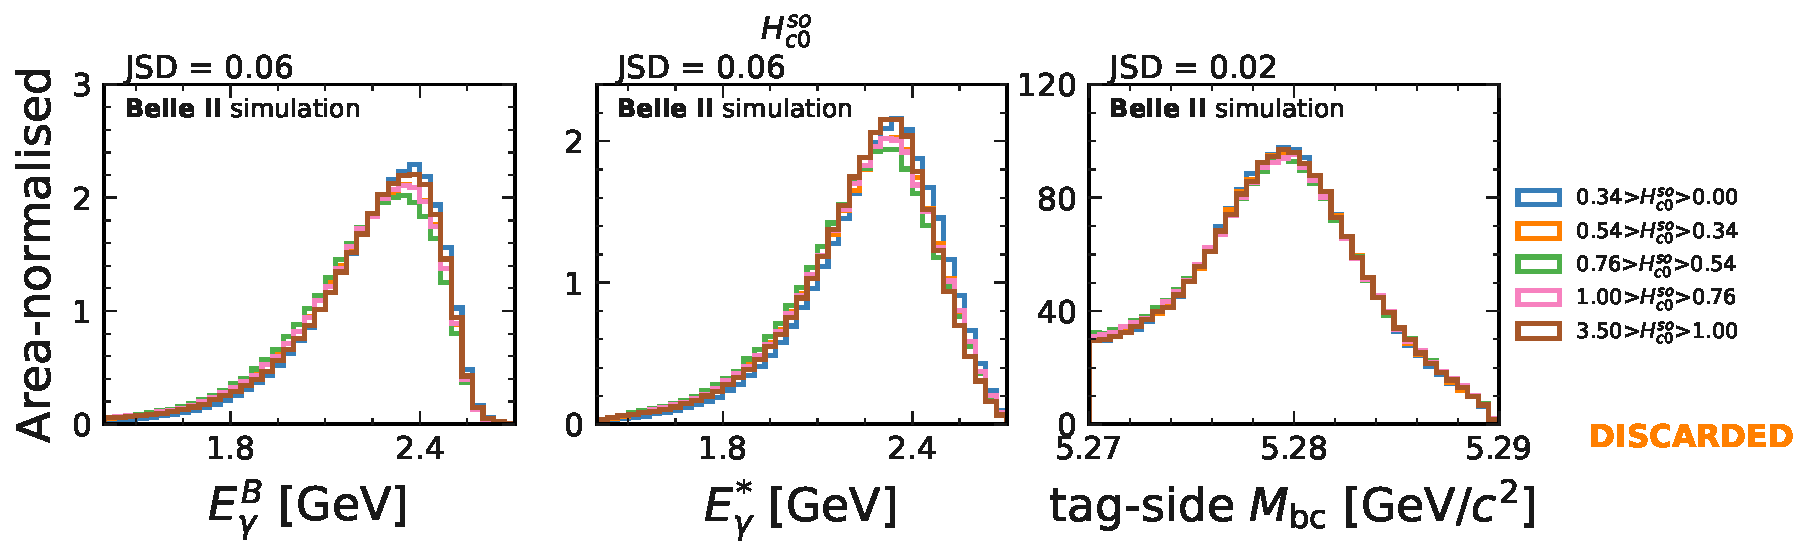
\includegraphics[width=0.95\textwidth]{figures/appendices/continuum_suppression_features/modified_fox_wolfram_moments/Btag_KSFW_hso00_bias_tested.pdf}
    }
    \subcaptionbox{\label{fig:Btag_KSFW_hso01}}{
        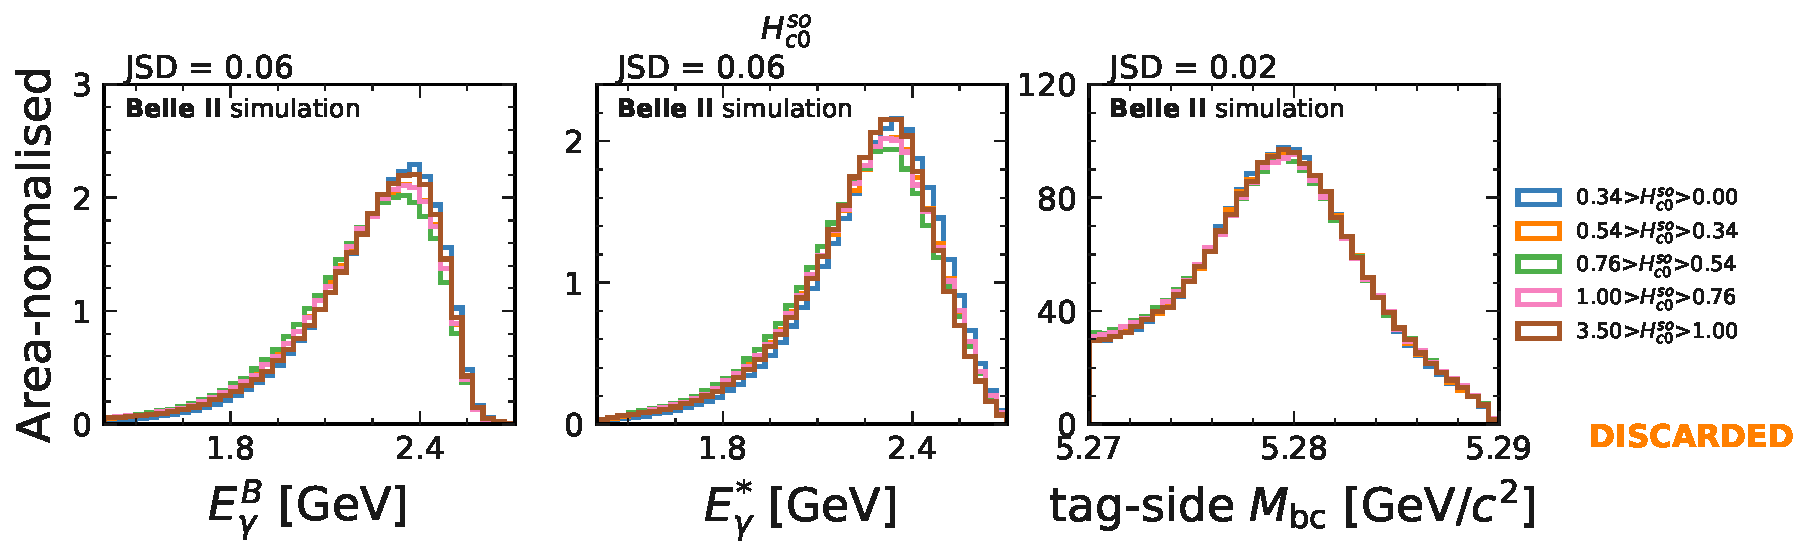
\includegraphics[width=0.95\textwidth]{figures/appendices/continuum_suppression_features/modified_fox_wolfram_moments/Btag_KSFW_hso00_bias_tested.pdf}
    }
    \subcaptionbox{\label{fig:Btag_KSFW_hso02}}{
        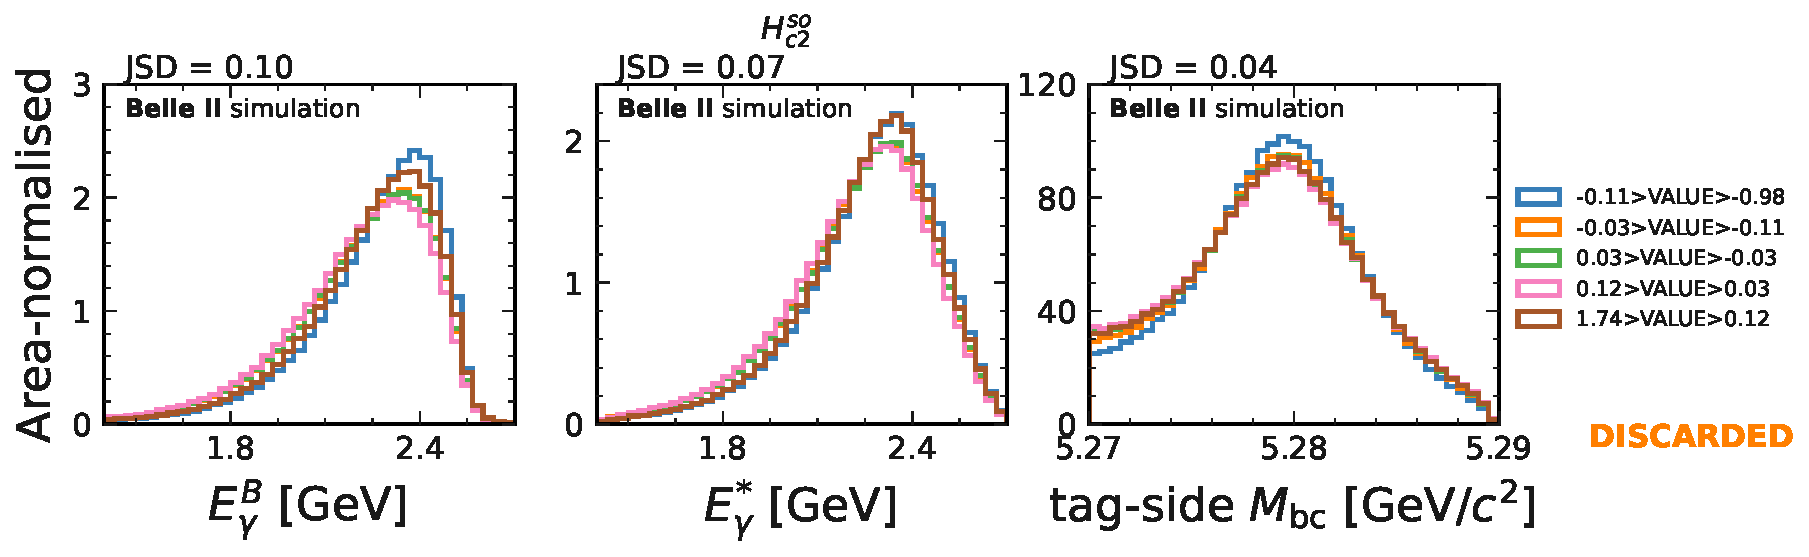
\includegraphics[width=0.95\textwidth]{figures/appendices/continuum_suppression_features/modified_fox_wolfram_moments/Btag_KSFW_hso02_bias_tested.pdf}

    }
    \subcaptionbox{\label{fig:Btag_KSFW_hso03}}{
        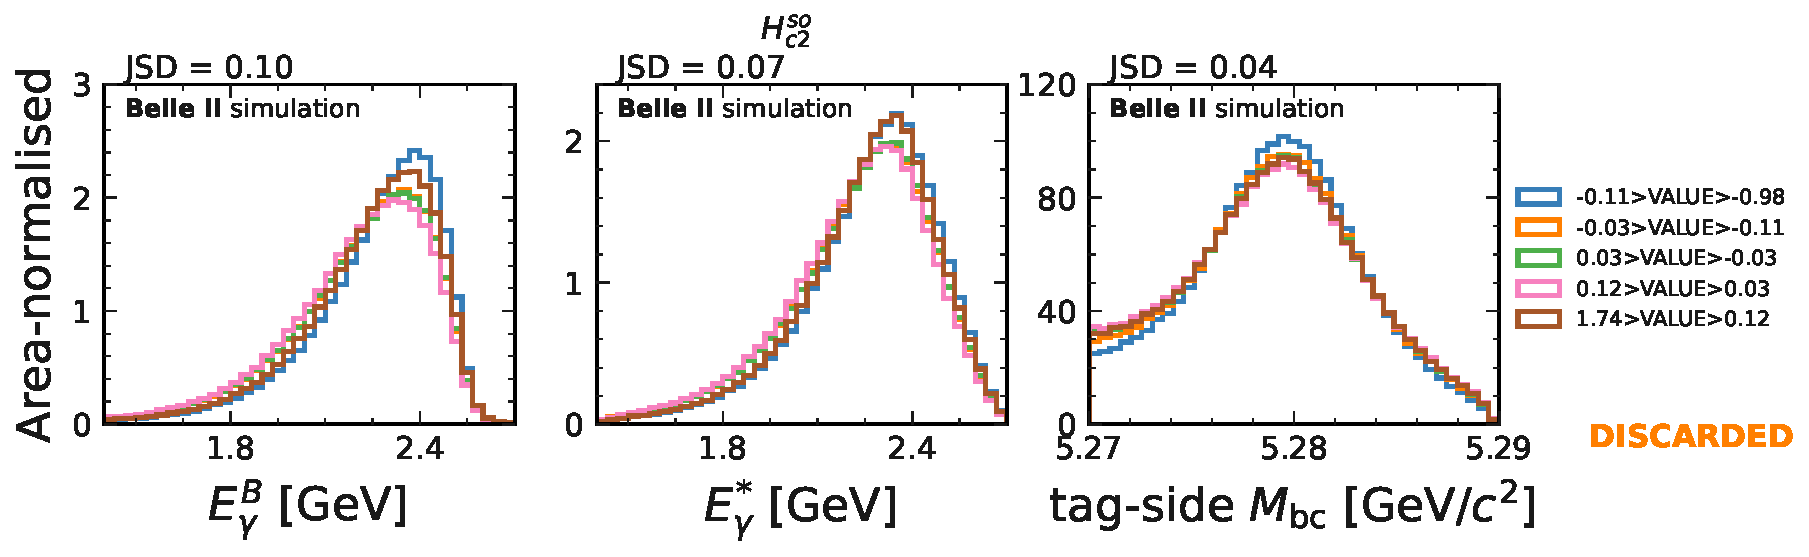
\includegraphics[width=0.95\textwidth]{figures/appendices/continuum_suppression_features/modified_fox_wolfram_moments/Btag_KSFW_hso02_bias_tested.pdf}

    }
\end{figure}
\begin{figure}[htbp!]
    \centering
    \ContinuedFloat
    \subcaptionbox{\label{fig:Btag_KSFW_hso04}}{
        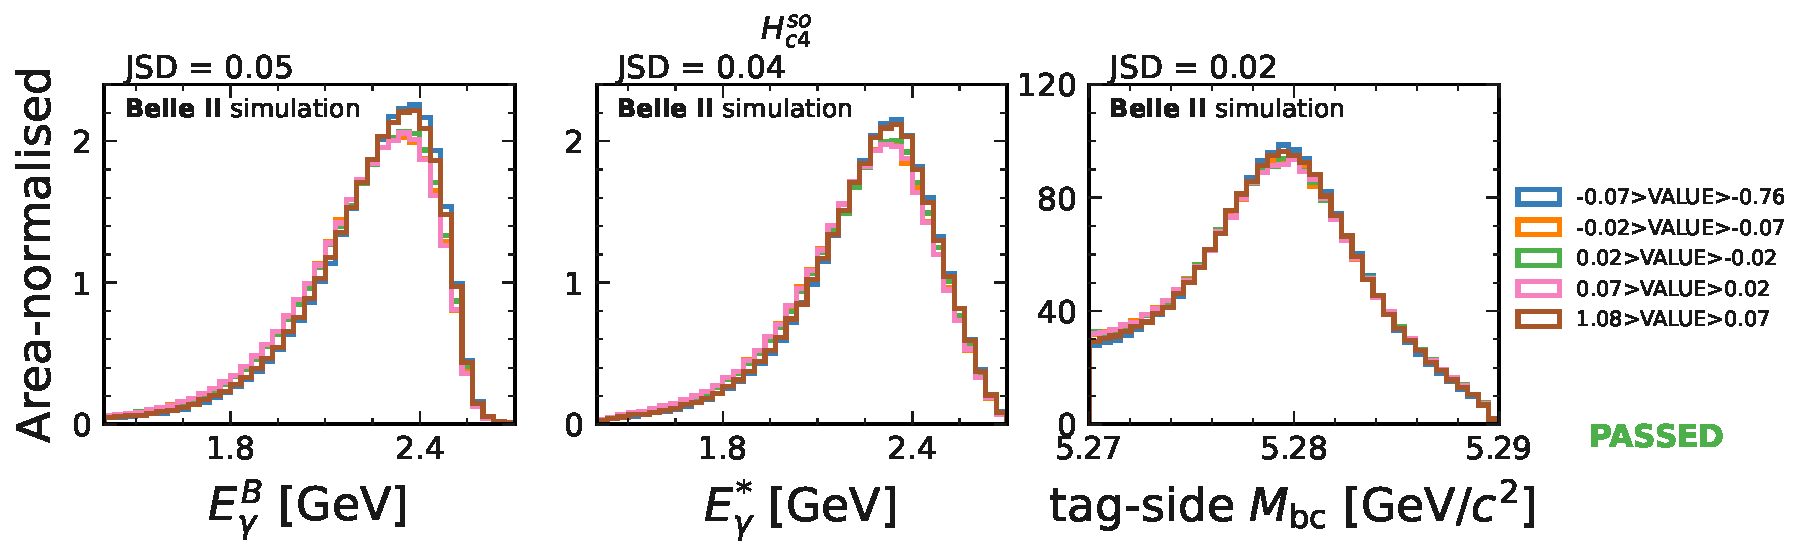
\includegraphics[width=0.95\textwidth]{figures/appendices/continuum_suppression_features/modified_fox_wolfram_moments/Btag_KSFW_hso04_bias_tested.pdf}

    }
    \subcaptionbox{\label{fig:Btag_KSFW_hso10}}{
        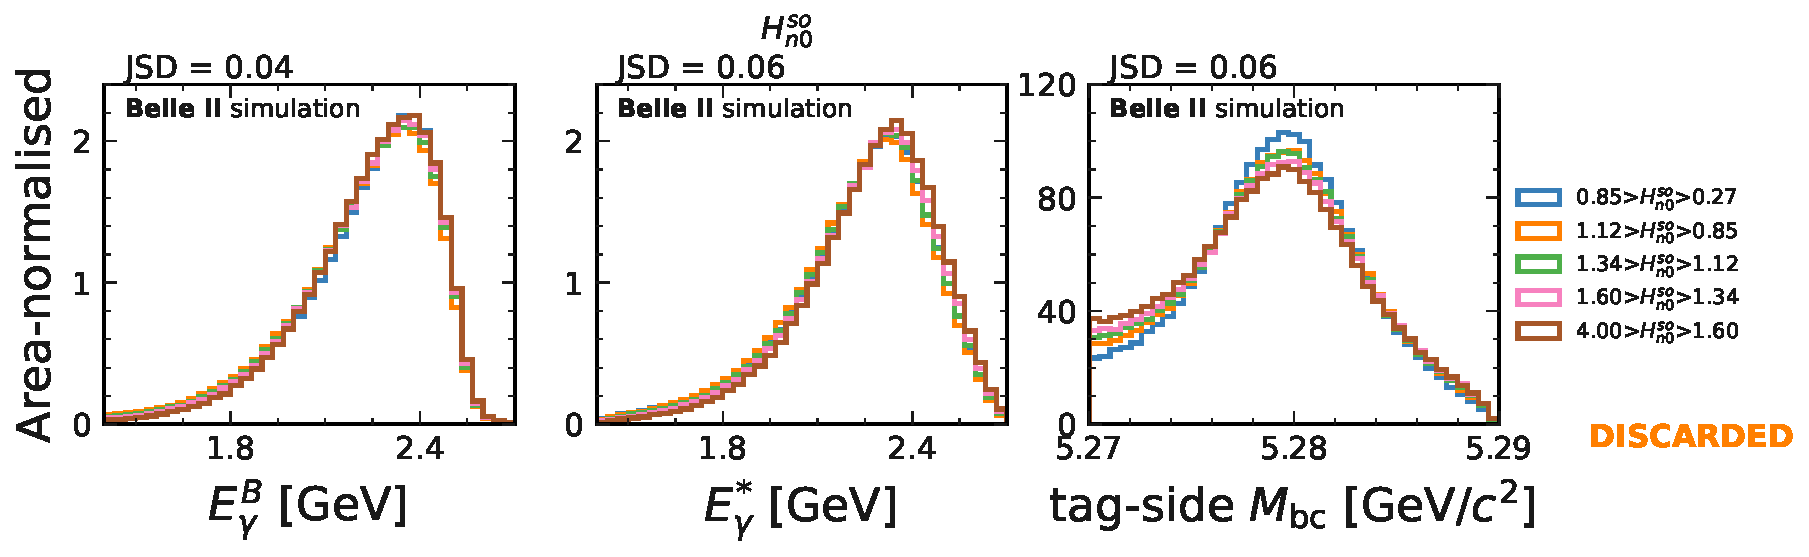
\includegraphics[width=0.95\textwidth]{figures/appendices/continuum_suppression_features/modified_fox_wolfram_moments/Btag_KSFW_hso10_bias_tested.pdf}

    }
    \subcaptionbox{\label{fig:Btag_KSFW_hso12}}{
        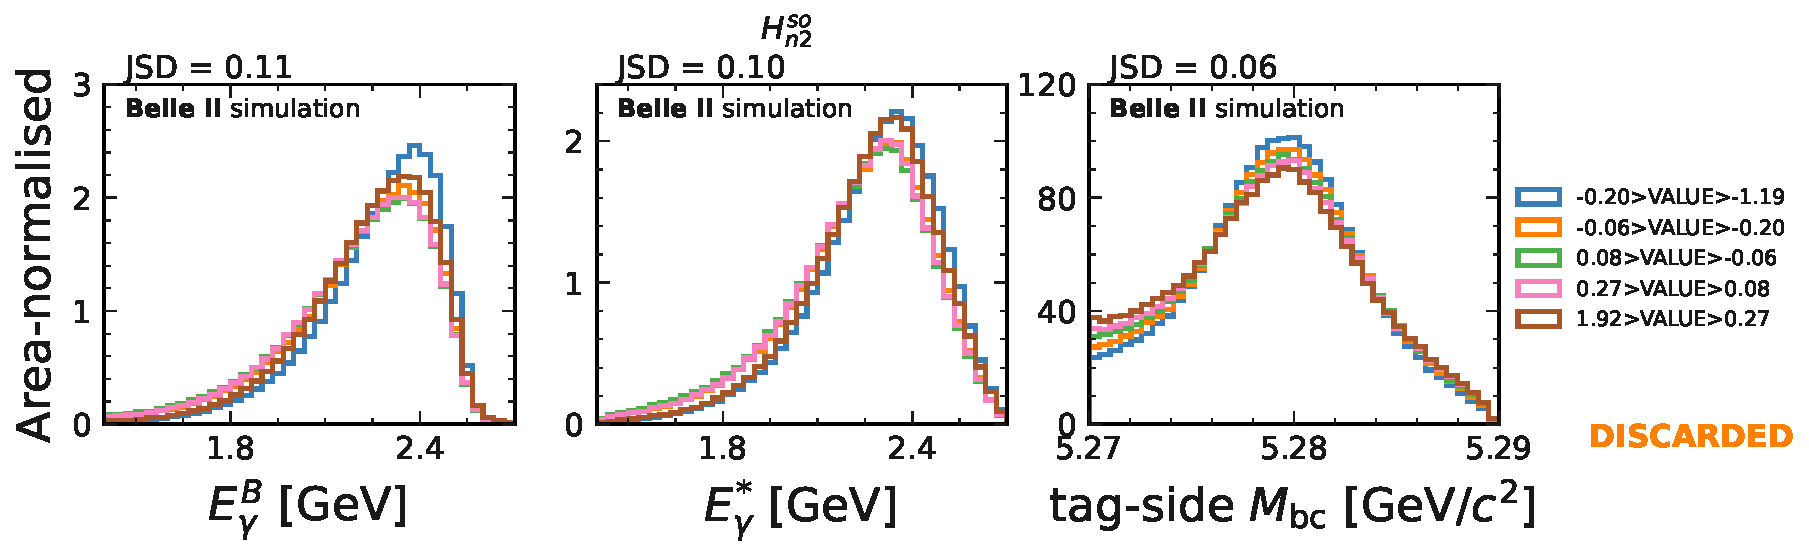
\includegraphics[width=0.95\textwidth]{figures/appendices/continuum_suppression_features/modified_fox_wolfram_moments/Btag_KSFW_hso12_bias_tested.pdf}

    }
    \subcaptionbox{\label{fig:Btag_KSFW_hso14}}{
        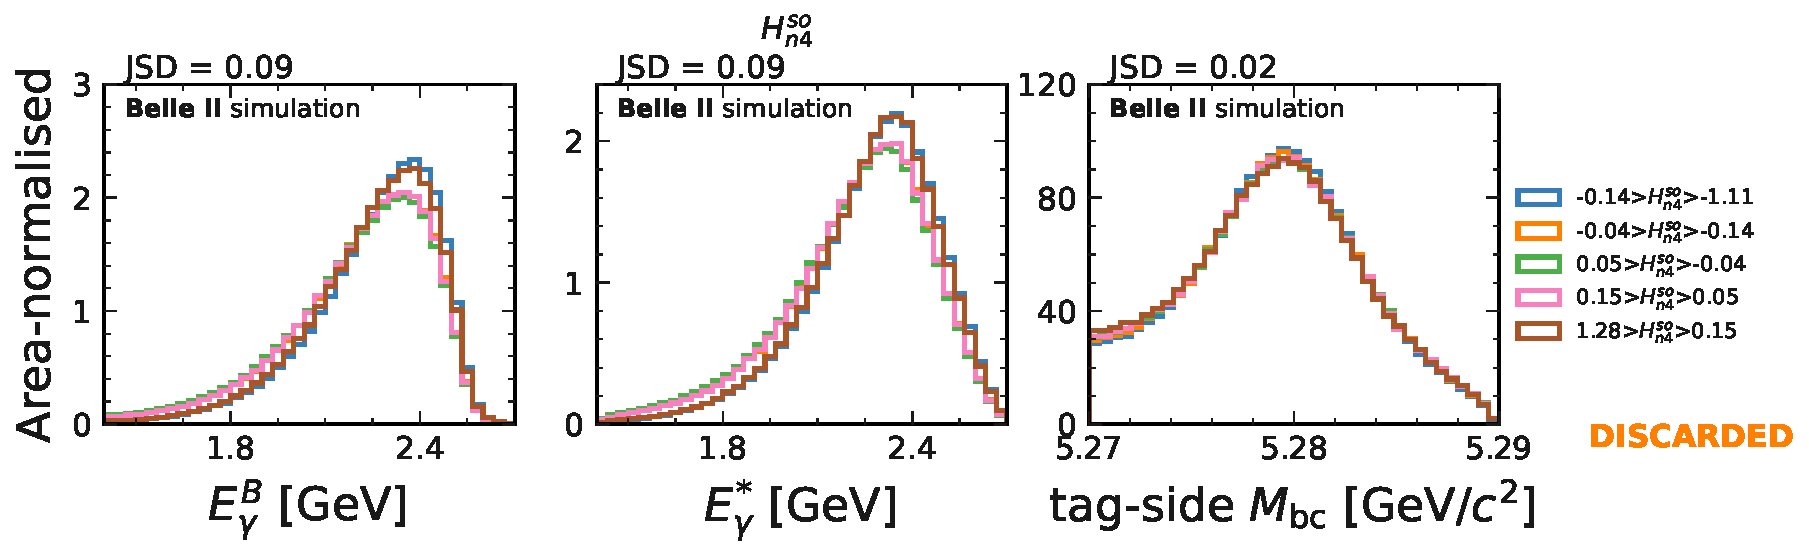
\includegraphics[width=0.95\textwidth]{figures/appendices/continuum_suppression_features/modified_fox_wolfram_moments/Btag_KSFW_hso14_bias_tested.pdf}

    }
\end{figure}
\begin{figure}[htbp!]
\centering
\ContinuedFloat
    \subcaptionbox{\label{fig:Btag_KSFW_hso20}}{
        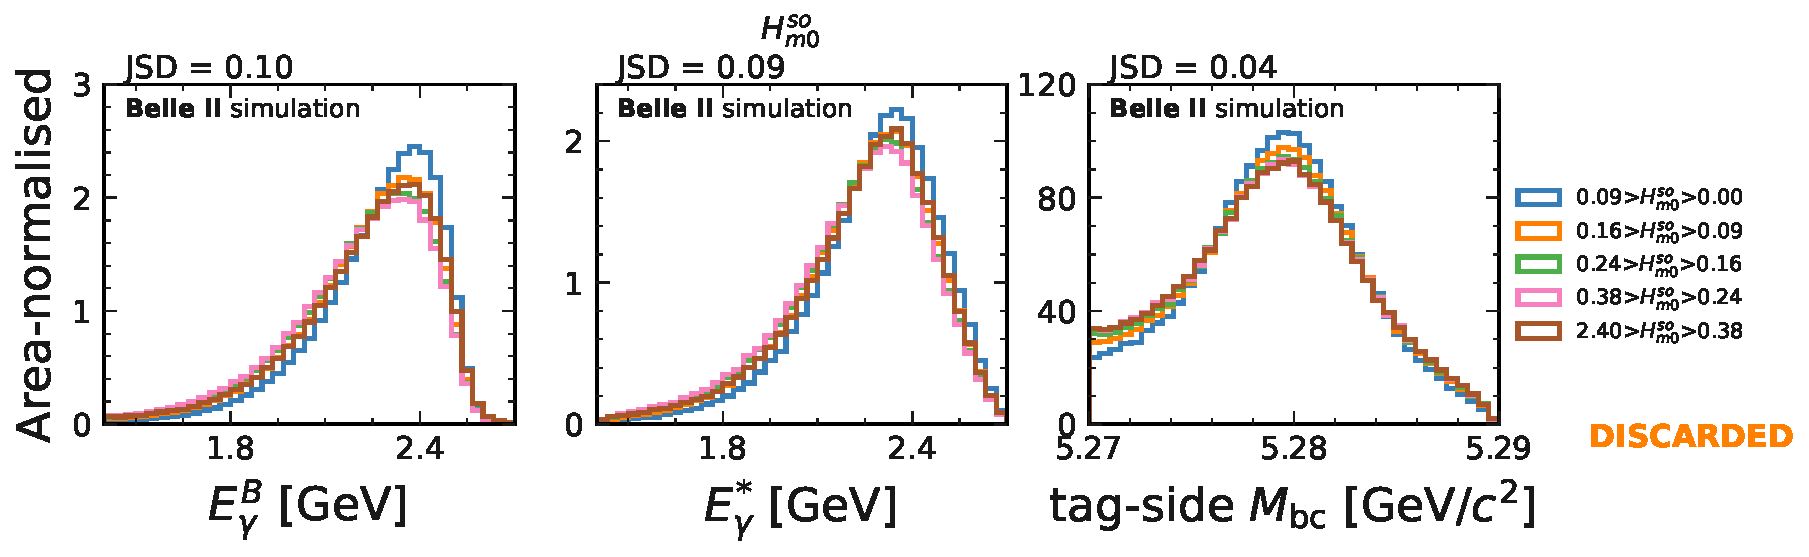
\includegraphics[width=0.95\textwidth]{figures/appendices/continuum_suppression_features/modified_fox_wolfram_moments/Btag_KSFW_hso20_bias_tested.pdf}

    }
    \subcaptionbox{\label{fig:Btag_KSFW_hso22}}{
        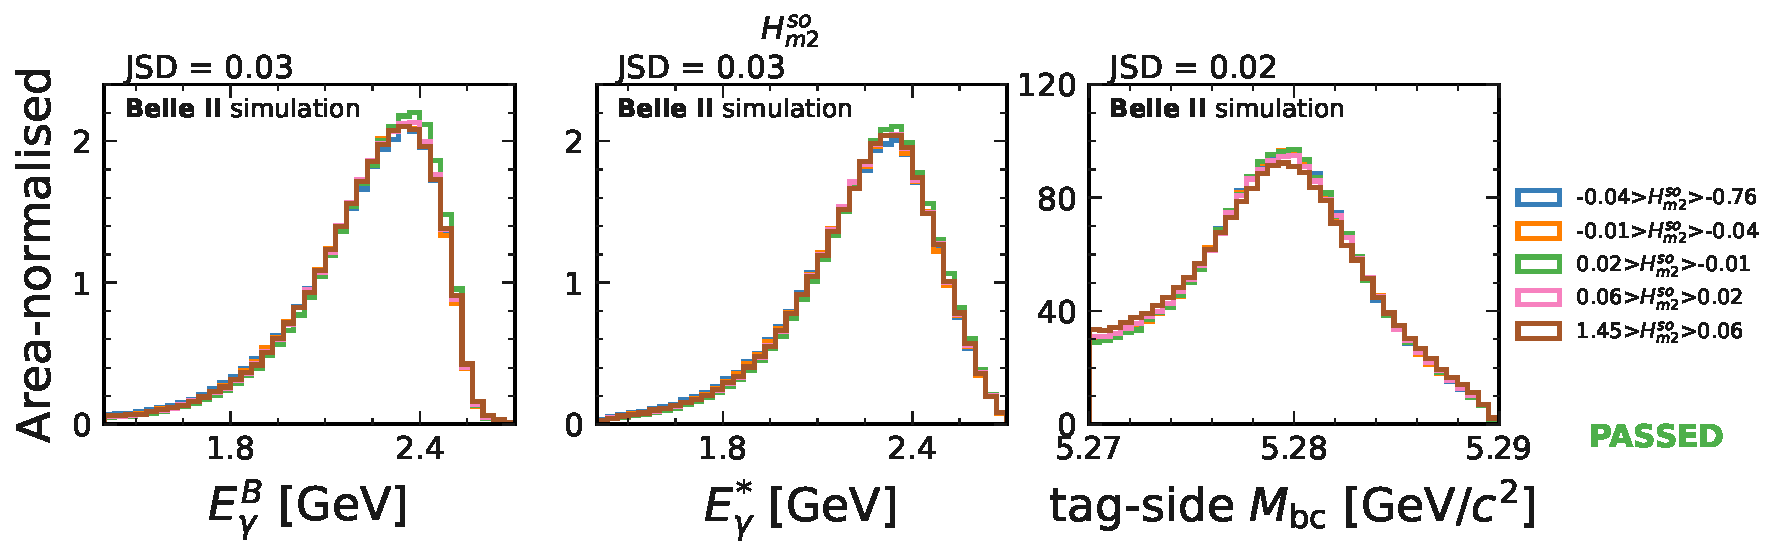
\includegraphics[width=0.95\textwidth]{figures/appendices/continuum_suppression_features/modified_fox_wolfram_moments/Btag_KSFW_hso22_bias_tested.pdf}

    }
    \subcaptionbox{\label{fig:Btag_KSFW_hso24}}{
        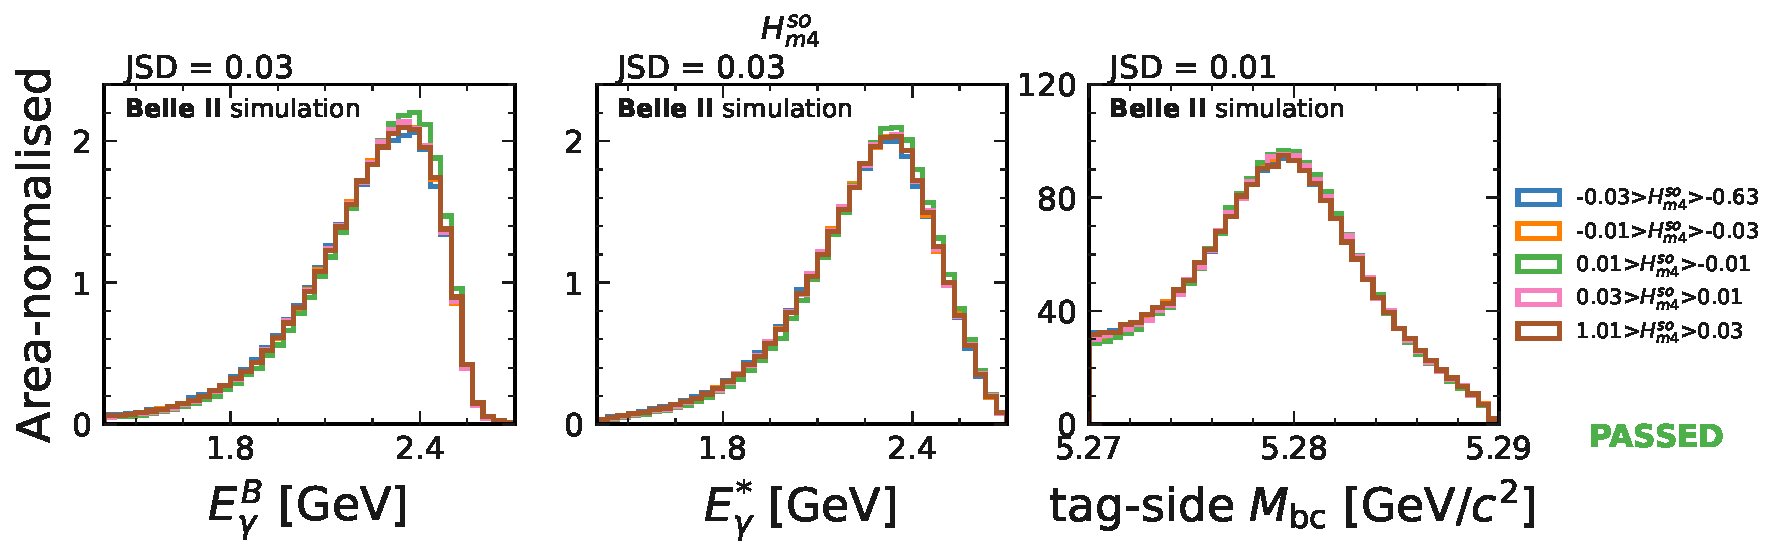
\includegraphics[width=0.95\textwidth]{figures/appendices/continuum_suppression_features/modified_fox_wolfram_moments/Btag_KSFW_hso24_bias_tested.pdf}

    }
    \subcaptionbox{\label{fig:Btag_KSFW_hoo0}}{
        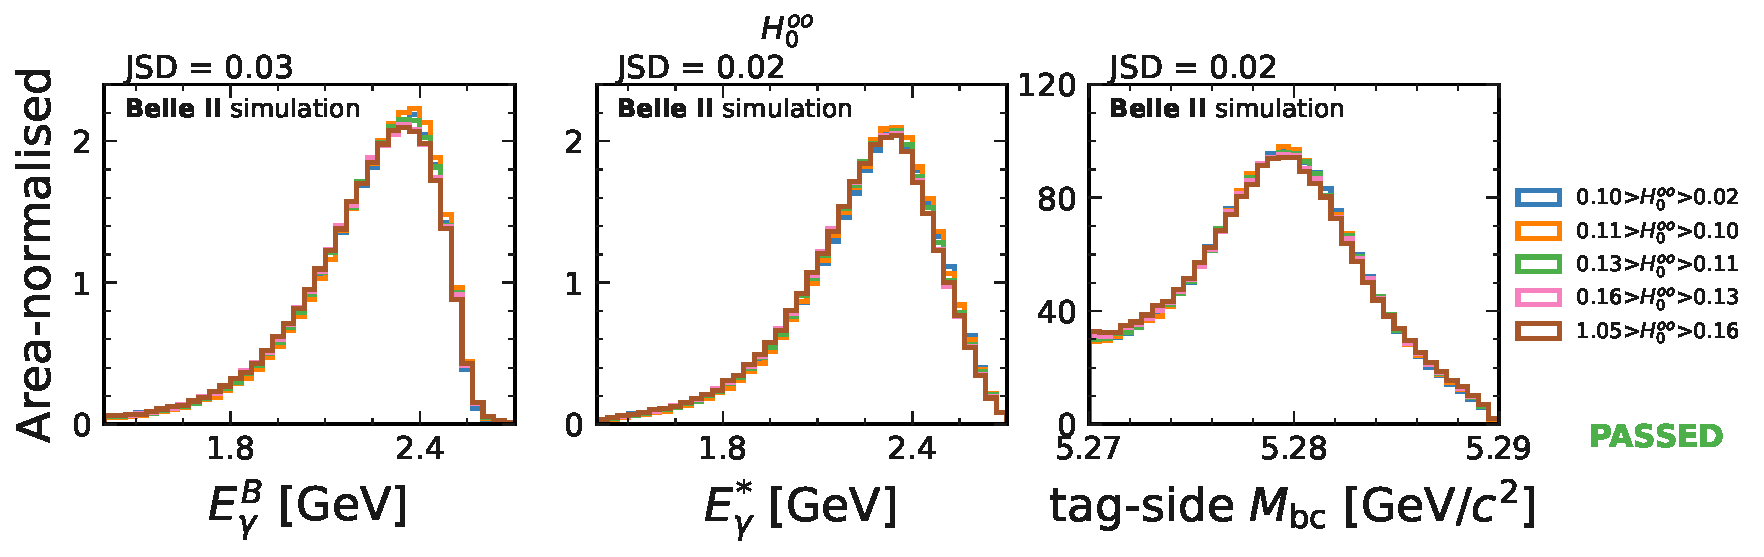
\includegraphics[width=0.95\textwidth]{figures/appendices/continuum_suppression_features/modified_fox_wolfram_moments/Btag_KSFW_hoo0_bias_tested.pdf}

    }
\end{figure}
\begin{figure}[htbp!]
    \centering
    \ContinuedFloat
    \subcaptionbox{\label{fig:Btag_KSFW_hoo1}}{
        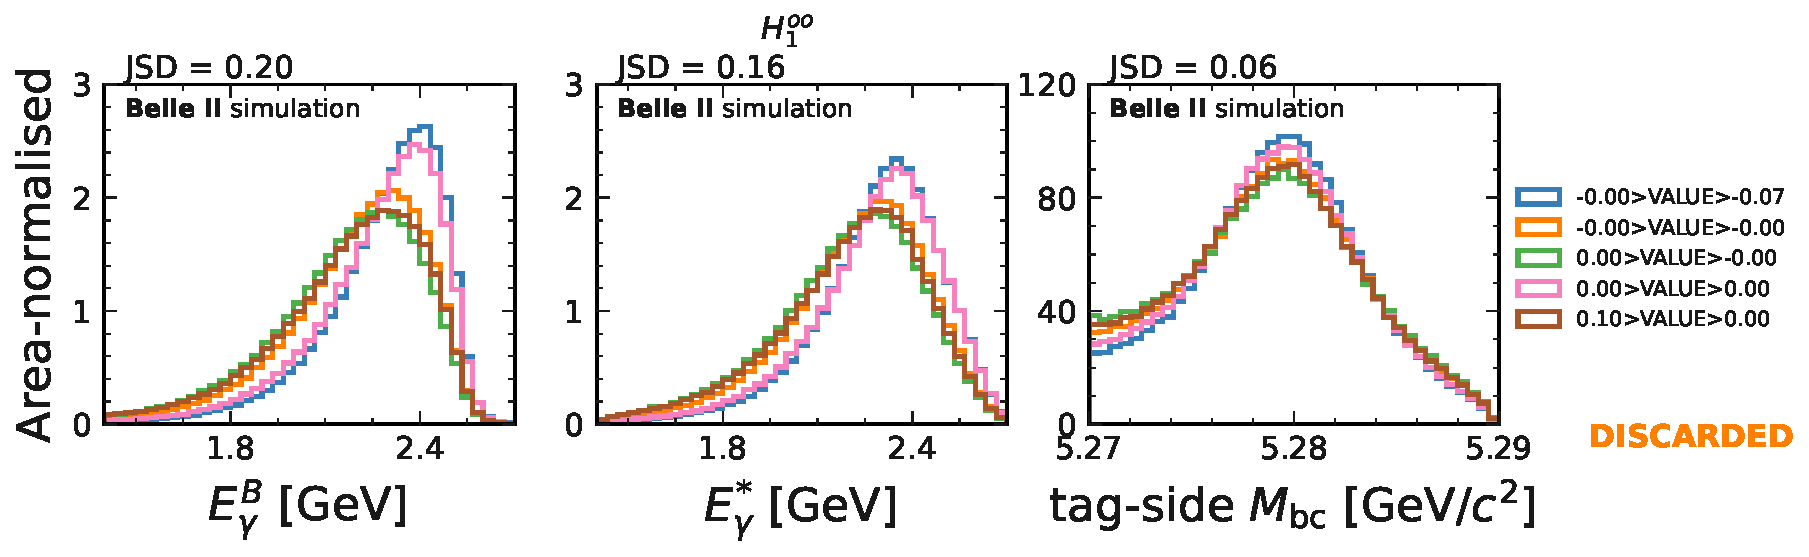
\includegraphics[width=0.95\textwidth]{figures/appendices/continuum_suppression_features/modified_fox_wolfram_moments/Btag_KSFW_hoo1_bias_tested.pdf}

    }
    \subcaptionbox{\label{fig:Btag_KSFW_hoo2}}{
        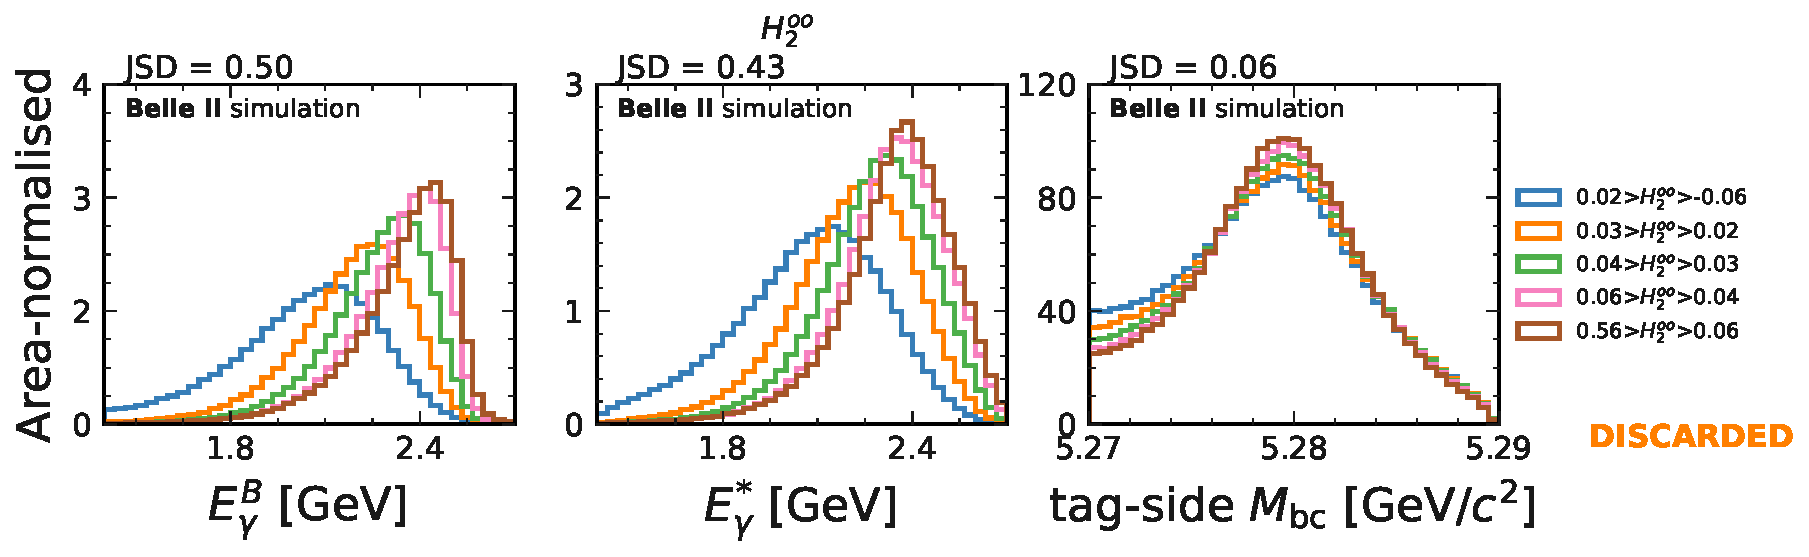
\includegraphics[width=0.95\textwidth]{figures/appendices/continuum_suppression_features/modified_fox_wolfram_moments/Btag_KSFW_hoo2_bias_tested.pdf}

    }
    \subcaptionbox{\label{fig:Btag_KSFW_hoo3}}{
        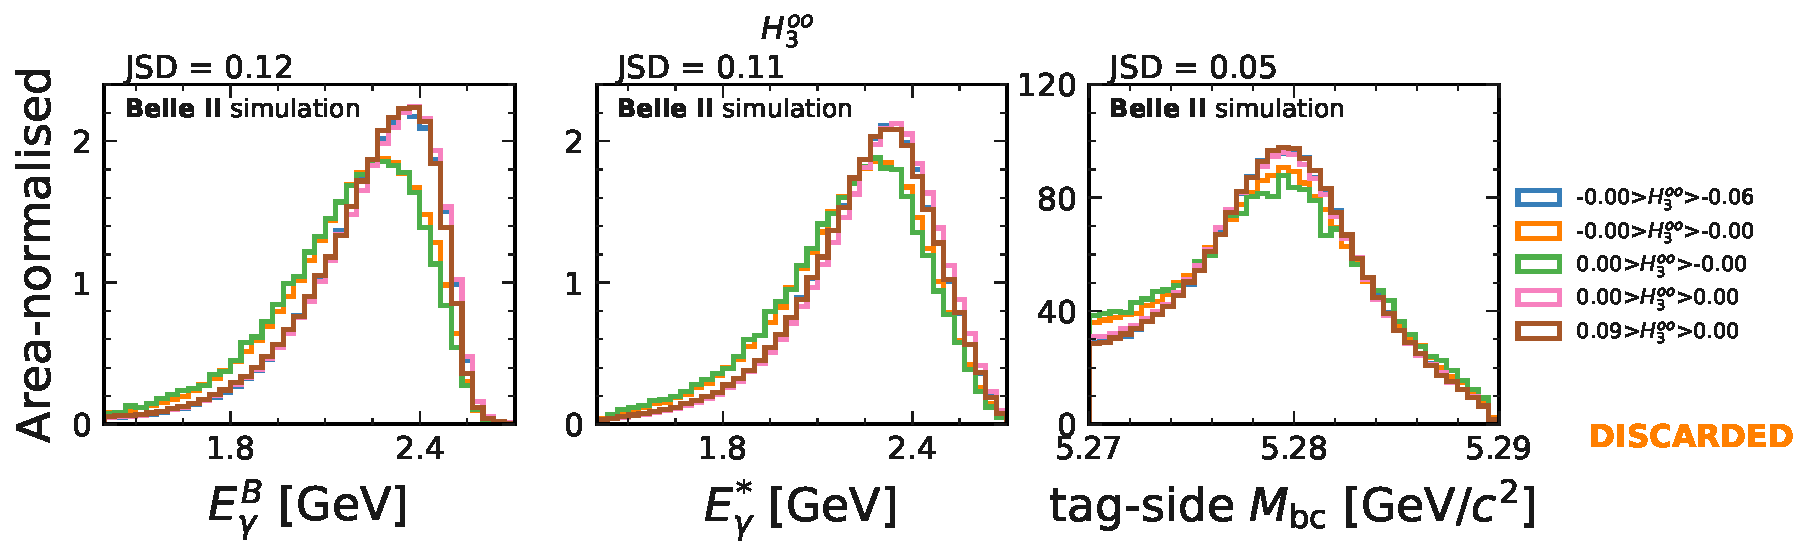
\includegraphics[width=0.95\textwidth]{figures/appendices/continuum_suppression_features/modified_fox_wolfram_moments/Btag_KSFW_hoo3_bias_tested.pdf}

    }
    \subcaptionbox{\label{fig:Btag_KSFW_hoo4}}{
        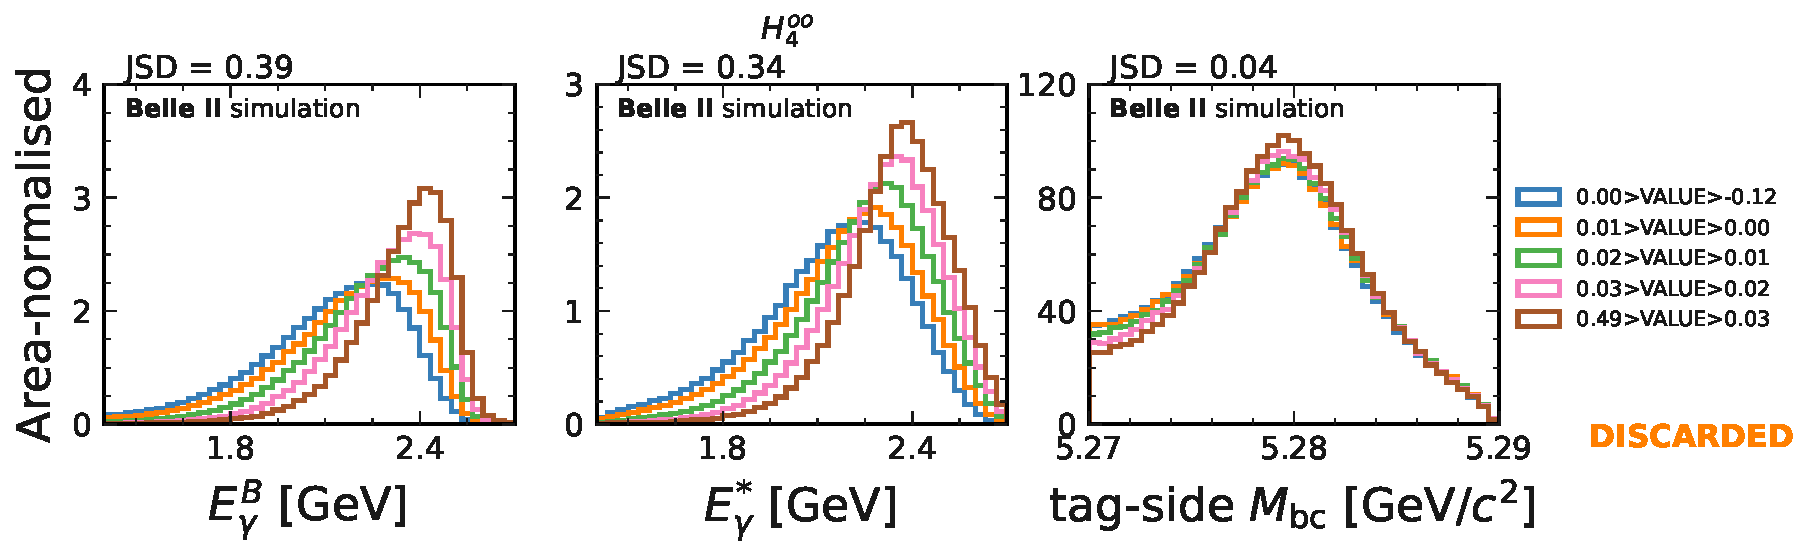
\includegraphics[width=0.95\textwidth]{figures/appendices/continuum_suppression_features/modified_fox_wolfram_moments/Btag_KSFW_hoo4_bias_tested.pdf}

    }

\end{figure}
\begin{figure}[htbp!]
    \centering
    \ContinuedFloat
\subcaptionbox{\label{fig:Btag_KSFW_et}}{
    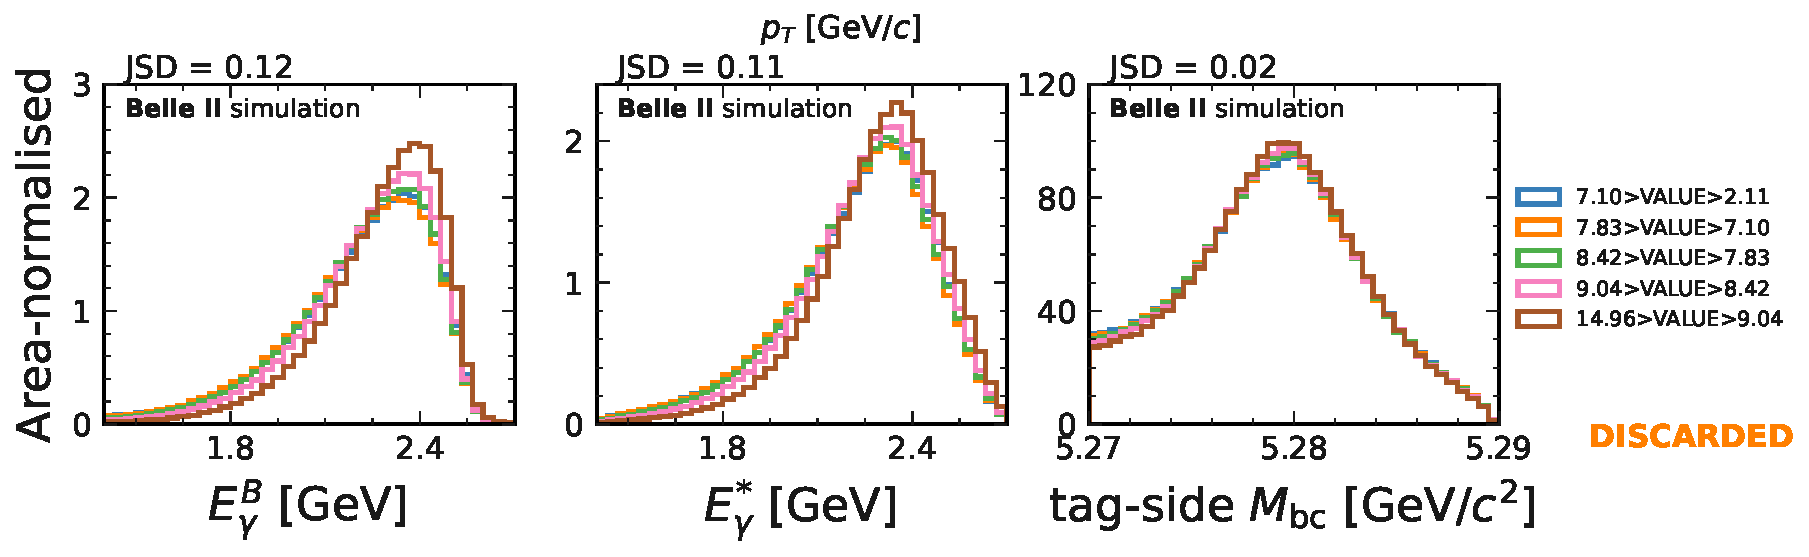
\includegraphics[width=0.95\textwidth]{figures/appendices/continuum_suppression_features/modified_fox_wolfram_moments/Btag_KSFW_et_bias_tested.pdf}

}
\subcaptionbox{\label{fig:Btag_KSFW_mm2}}{
    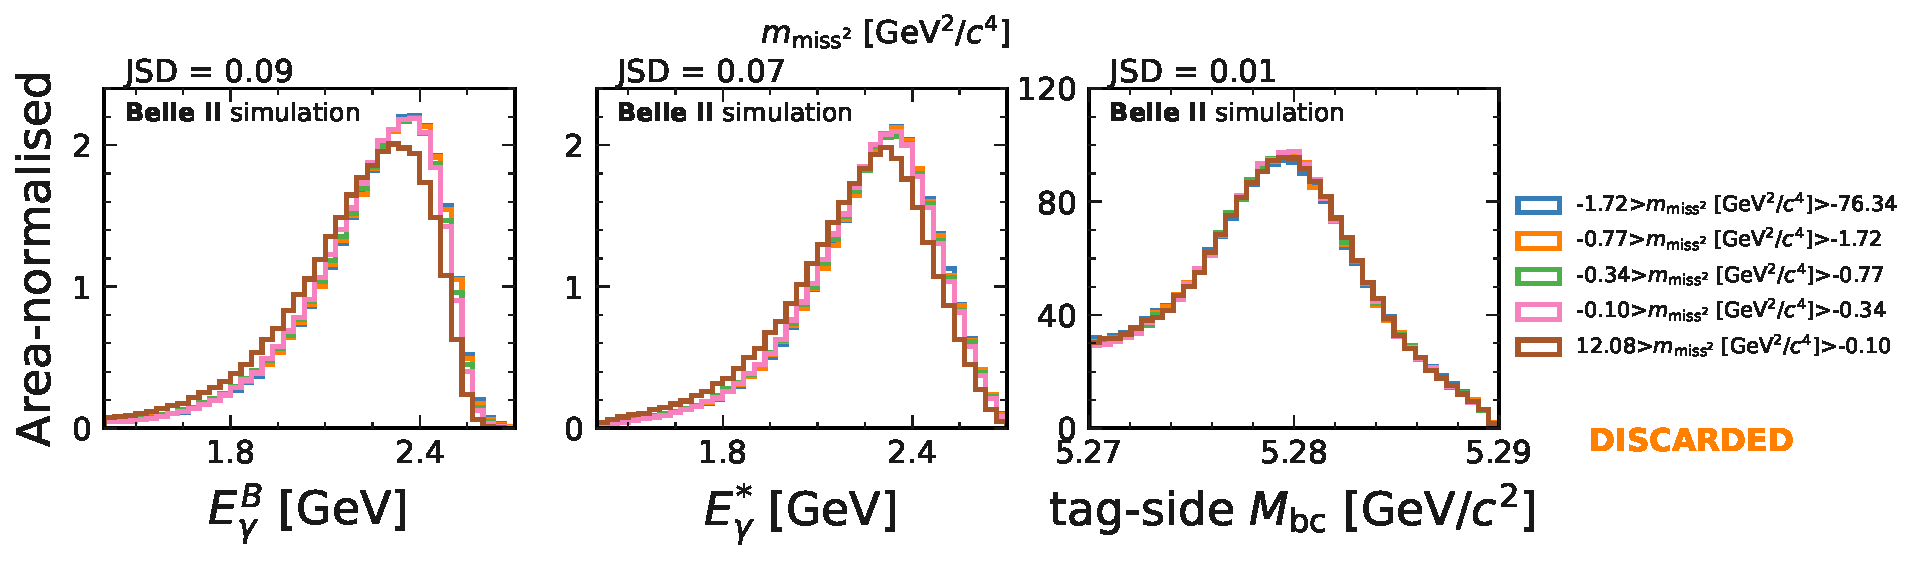
\includegraphics[width=0.95\textwidth]{figures/appendices/continuum_suppression_features/modified_fox_wolfram_moments/Btag_KSFW_mm2_bias_tested.pdf}

}
\caption{\label{fig:modified_fox_wolframs_test1} The bias-test on \EB, \Estar and \Mbc for modified Fox-Wolfram moments.
The test is performed based on \textbf{Test~1} strategy, defined in \Cref{sec:continuum_features}.
Variable definitions are given in the text.}
\end{figure}
